\section{Experimental Evaluation} 
\label{sec:experiments}

%This section presents the research questions and the experiments we conducted and analyzed to validate our approximate distributed monitoring approach.

%\subsection{Research Questions}

We seek answers to the following research questions (RQs):
%\vspace{-0.25em}
\begin{resq}[What is the tradeoff between the efficiency and the accuracy of approximate distributed monitors?]
The approximate distributed monitoring comes with a price in terms of the loss of accuracy.
We want to understand the tradeoff between the potential speedups that an approximate distributed monitor can achieve when compared to its exact counterpart and the consequent loss in accuracy due to the approximations.
We would also like to identify the classes of signals and properties for which this tradeoff is effective. 
\end{resq}
%\vspace{-0.75em}
\begin{resq}[Can the combination of approximate and exact distributed monitors increase efficiency while preserving accuracy?]
We are interested in evaluating whether a smart, combined use of approximate and exact distributed monitors can still bring improvements in monitoring efficiency while guaranteeing the accuracy of the monitoring verdicts. 
\end{resq}
\bgroup \color{red}
\begin{resq}[How scalable are online incremental monitors?]
The offline monitors can be naively used for online monitoring, which comes with immediate soundness but computational overhead due to redundant computation and using memory carelessly.
The alternative, incremental monitoring approach aims to address these issues.
We want to understand to which degree the incremental approach achieves this goal and scales to scenarios with high-frequency sampling and large clock skew.
\end{resq}
\egroup

\begin{table*}[t]
	\centering
	%	\scalebox{0.88}{
		\begin{tabular}{|l|l|}
			\hline
			Subject & STL formula(s) \\
			\hline
			%			RG & $\varphi_1 =\LTLg (p \wedge q)$ \,\,\,\,\,\, $\varphi_2 = \LTLg (p \Rightarrow \LTLf q)$ \,\,\,\,\,\, $\varphi_3 = \LTLg (p \Rightarrow \LTLf_{[0,1)} q)$ \\
			%			   & $\varphi_4 = \LTLg (p \lor q)$ \,\,\,\,\,\,  $\varphi_5 = p \until q$ \,\,\,\,\,\, $\varphi_6 = \LTLg (p \Rightarrow \LTLf_{[0,2)} q)$ \\
			RG (offline) & $\varphi_1 =\LTLg (p \wedge q)$ \,\,\,\,\,\,\,\,\,\,\,\,\,\,\, $\varphi_2 =\LTLg (p \lor q)$ \,\,\,\,\,\,\,\,\,\,\,\,\,\,\,\,\,\,\,\,\,\,\,\,\, $\varphi_3 = p \until q$ \\
			& $\varphi_4 = \LTLg (p \Rightarrow \LTLf q)$  \,\,\,\,\,\,  $\varphi_5 = \LTLg (p \Rightarrow \LTLf_{[0,1)} q)$ \,\,\,\,\,\, $\varphi_6 = \LTLg (p \Rightarrow \LTLf_{[0,2)} q)$ \\
			RG (online) & $\psi_1 =\LTLsquareminus (p \wedge q)$ \,\,\,\,\,\,\,\,\,\,\,\,\,\,\, $\psi_2 =\LTLsquareminus (p \lor q)$ \,\,\,\,\,\,\,\,\,\,\,\,\,\,\,\,\,\,\,\,\,\,\,\,\, $\psi_3 = p \since q$ \\
			& $\psi_4 = \LTLsquareminus (p \Rightarrow \LTLdiamondminus q)$  \,\,\,\,\,\,  $\psi_5 = \LTLsquareminus (p \Rightarrow \LTLdiamondminus_{[0,1)} q)$ \,\,\,\,\,\, $\psi_6 = \LTLsquareminus (p \Rightarrow \LTLdiamondminus_{[0,2)} q)$ \\
			%& $\varphi_1$ & $\LTLg (p \wedge q)$ & \multirow{ 5}{*}{untimed} \\
			%& $\varphi_2$ & $\LTLf (p \vee q)$ & \\
			%& $\varphi_3$ & $\LTLg (p \vee q)$ & \\
			%& $\varphi_4$ & $\LTLf (p \wedge q)$ & \\
			%& $\varphi_5$ & $p \until q$ & \\
			%			\hline
			WT & $\varphi_{\text{WT}} = \LTLg \left(\sum_{i=1}^{n} x_i  > c\right)$  \\
			%			\hline
			SD & $\varphi_{\text{SD}} = \bigwedge_{1 \leq i \neq j \leq n} \LTLg \left( \sqrt{(x_i-x_j)^2 + (y_i-y_j)^2 + (z_i-z_j)^2} > c \right)$   \\
			\hline
		\end{tabular}%}
	\caption{STL specifications used in the experiments.}
	%	\vspace{-3em}
	\label{tab:spec} 
\end{table*}

\subsection{Experimental Setup}

\paragraph*{Distributed Monitors.}
In our study, we compare our approximate distributed monitoring (\textsc{Adm}) approach and its variants to an exact distributed monitoring approach (\textsc{Edm}).\footnote[1]{The code is available at \url{https://github.com/egesarac/ApxDistMon}.}
For \textsc{Edm}, we take a variant of the distributed monitoring procedure from~\cite{MomtazAB23} that allows to evaluate STL specifications over distributed traces using SMT-solving.
Originally, that procedure assumes that input signals are polynomial continuous functions.
We adapt the SMT-based approach to consider input signals as piecewise-constant signals to make a consistent comparison with \textsc{Adm}.
We note that the passage from the polynomial continuous to piecewise-constant input signals reduces the efficiency of the SMT-based monitors.
We also observe that the SMT-based monitors from~\cite{MomtazAB23} can split the input trace into multiple segments and evaluate the specification incrementally, segment-by-segment, allowing early termination of the monitor in some cases.
Since the focus of this comparison is purely on the offline monitoring, we also use the exact monitors without their incremental mode.
%We use the abbreviation \textsc{Edm} to denote the variant of the exact SMT-based distributed monitors used in this study.


%\vspace{-0.35em}
\paragraph*{Experimental Subjects.}
To answer our research questions, we use (1) a \emph{random generator (RG)} of distributed traces, (2) a \emph{water tank (WT)} case study, and (3) a \emph{swarm of drones (SD)} case study.  
%
\emph{The random generator (RG)} uses uniform distribution to generate distributed traces, in which the user can control the duration $d$ of the trace, as well as the $\varepsilon$ bound on the uncertainty at which the events happen.
\emph{Water tank (WT)} model is a SimuLink model of a hybrid high pressure water distribution system consisting of two water tanks. Inlet pipes connect each water tank to an external source, and outlet pipes distribute high pressure water that is regulated by valves.
Each valve is operated by a controller that samples the outflow pressure at 20Hz using its local clock. Our model is a simplified emulation of the Refueling Water Storage Tanks (RWST) module of an Emergency Core Cooling System (ECCS) of a Pressurized Water Reactor Plant~\cite{USNRCPWR}.
\emph{Swarm of drones (SD)} model is generated using a path planning software, Fly-by-Logic~\cite{PantAM17CCTA}. Here, a swarm of drones perform various reach-avoid missions, while securing objectives such as reaching a goal within a deadline, avoiding obstacles and collisions. The path planner finds the most robust trajectory using a temporal logic robustness optimizer. These trajectories are sampled at 20Hz.
Note that the actual values of clock skew are less important than the fact that when clock skew exceeds the sampling interval, we encounter the problem of uncertainty.



%\vspace{-0.4em}
\paragraph*{Specifications.}
Table~\ref{tab:spec} shows the STL specifications that we use to evaluate our experimental subjects.
For offline monitoring, specifications $\varphi_{1}$ to $\varphi_{6}$ are monitored against the distributed traces created by the random generator and represent different classes and fragments of Boolean-valued temporal formulas.
The specification $\varphi_1$ is an LTL formula in which both the outer temporal operator ($\LTLg$) and the inner Boolean operator ($\wedge$) are conjunctive.
The specification $\varphi_2$ combines conjunctive $(\LTLg)$ and disjunctive ($\lor$) operators, and $\varphi_3$ is the usual until operator.
The remaining three formulas are the common response formulas, which also combine conjunctive $(\LTLg)$ and disjunctive $(\LTLf, \Rightarrow)$ operators: $\varphi_4$ is the usual LTL variant, $\varphi_5$ and $\varphi_6$ add a bounded real-time response requirement to the previous specification, where the bound of $\varphi_5$ is tighter than that of $\varphi_6$.
For online monitoring, we use the past-time variants $\psi_1$ to $\psi_6$ of the formulas described above.
The specification $\varphi_{WT}$ associated to the water tank case study is an STL formula in which a sum of signals originating from different agents is compared to a constant. Finally, the specification $\varphi_{SD}$ defines a mutual separation property over a swarm of drones, requiring more sophisticated arithmetic operations on signals originating from different agents.

%\begin{table}[t]
%\centering
%\scalebox{0.85}{
%\begin{tabular}{|l|l|l|l|}
%\hline
%Subject & Spec ID & STL formula \\
%\hline
%\multirow{3}{*}{RG}
%& $\varphi_1$ & $\LTLg (p \wedge q)$  \\
%& $\varphi_2$ & $\LTLg (p \Rightarrow \LTLf q)$ \\
%& $\varphi_3$ & $\LTLg (p \Rightarrow \LTLf_{[0,1)} q)$  \\
%%& $\varphi_1$ & $\LTLg (p \wedge q)$ & \multirow{ 5}{*}{untimed} \\
%%& $\varphi_2$ & $\LTLf (p \vee q)$ & \\
%%& $\varphi_3$ & $\LTLg (p \vee q)$ & \\
%%& $\varphi_4$ & $\LTLf (p \wedge q)$ & \\
%%& $\varphi_5$ & $p \until q$ & \\
%\hline
%WT & $\varphi_{\text{WT}}$ & $\LTLg \left(\sum_{i=1}^{n} x_i  > c\right)$  \\
%SD & $\varphi_{\text{SD}}$ & $\bigwedge_{1 \leq i \neq j \leq n} \LTLg \left( \sqrt{(x_i-x_j)^2 + (y_i-y_j)^2 + (z_i-z_j)^2} > c \right)$   \\
%\hline
%\end{tabular}}
%\caption{STL specifications used in the experiments.}
%\vspace{-3em}
%\label{tab:spec} 
%\end{table}

%\vspace{-0.4em}
\paragraph*{Computing Platform.}
We used a laptop with Ubuntu 24.04, an AMD Ryzen 7 4800HS CPU at 2.90GHz clock rate, and 16GB of RAM.
\textsc{Adm} is implemented in C++ and compiled using \texttt{g++} version 13.2.0 with the optimization flag \texttt{-O3} enabled, and \textsc{Edm} invokes the SMT-solver Z3 \cite{MouraB08} and is based on \cite{MomtazAB23}.

\subsection{Discussion}

\begin{figure*}[t]
	\begin{center}
		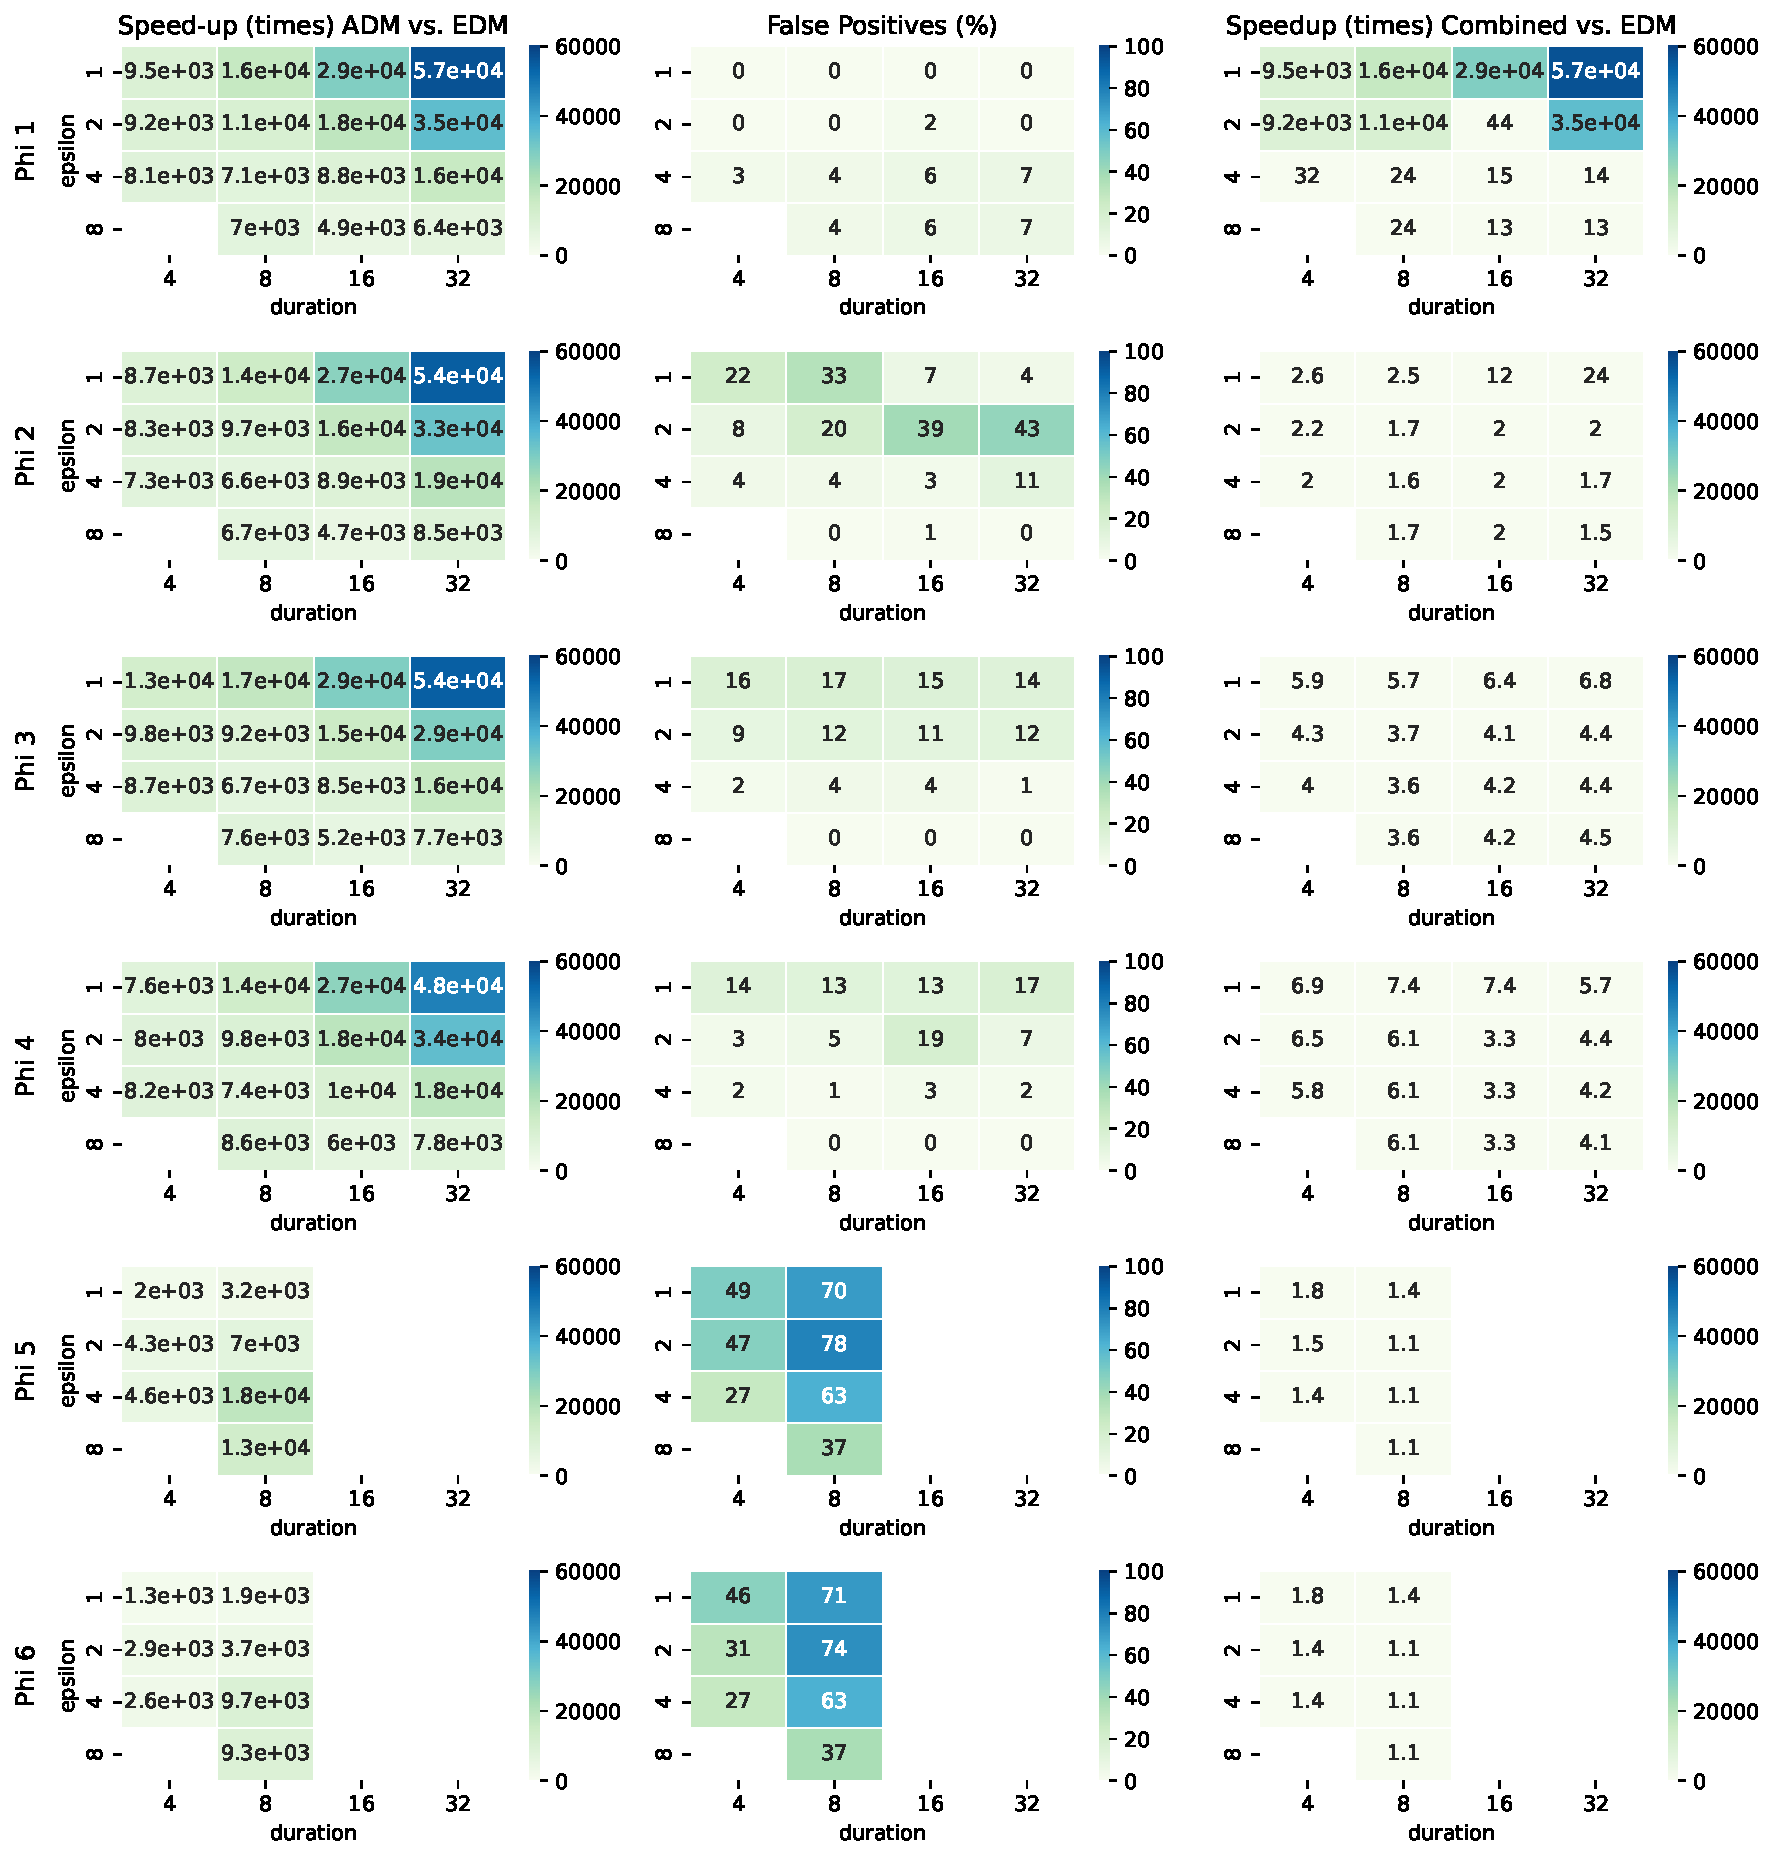
\includegraphics[width=\linewidth]{speedup_all}
		\caption{Results on monitoring $\varphi_{1}$ to $\varphi_{6}$ on distributed traces created by the RG.}
		\label{fig:rgresults}
	\end{center}
	%\vspace{1em}
\end{figure*}


%\vspace{-0.3em}
\paragraph*{Random Generator, Offline Monitoring.}
Figure~\ref{fig:rgresults} summarizes the results of evaluating specifications $\varphi_1$ to $\varphi_6$ against distributed traces from RG.
The first column in the figure depicts a heatmap where cells show the speedup of \textsc{Adm} compared to \textsc{Edm} when evaluating the formula on the given distributed trace with duration $d$ and uncertainty bound $\varepsilon$.
The second column shows a heatmap where every cell shows the percentage of \emph{false positives} (FP) introduced by \textsc{Adm}, where \textsc{Adm} evaluates to inconclusive when the \textsc{Edm} (real) verdict is true or false.
Finally, the third column depicts a heatmap, where each cell estimates the achieved speedup when combining \textsc{Adm} with \textsc{Edm}, compared to using only \textsc{Edm}.


We see that \textsc{Adm} consistently achieves speedups of \emph{several orders of magnitude} 
compared to the \textsc{Edm} approach.
The speedups range from several thousands to almost 60 thousand times, regardless of the considered specification, the duration $d$ of the trace, or the uncertainty bound $\varepsilon$.
These speedups and are the highest for long signals with low uncertainty bounds.
The price paid in terms of accuracy highly depends on the type of specification and the uncertainty bounds.
For example, \textsc{Adm} is very accurate when monitoring the property $\varphi_1$ in which both the temporal and the combinatorial operators are conjunctive.
On the other hand, having a combination of conjunctive and disjunctive operations (as in $\varphi_{2}$ and $\varphi_{4}$) increases the number of FPs.
Surprisingly, we see that in these cases the introduction of FPs is higher for lower values of $\varepsilon$.
This is because even \textsc{Edm} gives many inconclusive verdicts for higher values of $\varepsilon$.
We see that adding real-time modalities to the temporal operators increases FPs.
Finally, we can see (Figure~\ref{fig:rgresults} right column) that by combining \textsc{Edm} and \textsc{Adm}, we consistently get better performance than by using \textsc{Edm} only, even in cases where \textsc{Adm} introduces a high percentage of FPs.

%The approximate monitoring approach \textsc{Adm} consistently achieves computational speedups of \emph{several orders of magnitude} over the exact approach \textsc{Edm}, ranging from thousands to nearly 60 thousand times, regardless of  These speedups are highest for long signals with low uncertainty bounds. The accuracy tradeoff depends on the specification type and uncertainty bounds. \textsc{Adm} is very accurate for the property $\varphi_1$ with conjunctive operators, but combining conjunctive and disjunctive operations (as in $\varphi_2$ and $\varphi_3$) increases false positives (FPs), surprisingly at lower $\varepsilon$ values in particular. This is because higher $\varepsilon$ values result in many inconclusive verdicts even for \textsc{Edm}. Adding real-time modalities to temporal operators also increases FPs. Finally, as shown in the third column of \cref{fig:rgresults}, combining \textsc{Edm} and \textsc{Adm} consistently improves performance, even when \textsc{Adm} introduces many FPs.

\begin{figure*}[t]
	\begin{center}
		%		\includegraphics[width=\linewidth]{speedup_online}
		\caption{Results on monitoring $\psi_1$ to $\psi_6$ on distributed traces created by the RG.}	\label{fig:rgresultsOnline}
	\end{center}
	%\vspace{1em}
\end{figure*}


\paragraph*{Random Generator, Online Monitoring.}
Figure~\ref{fig:rgresultsOnline} summarizes the results of evaluating specifications $\psi_1$ to $\psi_6$ against distributed traces from RG.
As expected, \textsc{Adm-Incr} consistently outperforms \textsc{Adm-Naive}.
The speedup grows with trace length regardless of the clock skew $\varepsilon$ and portion size $\Delta$ values.
The largest gains occur for the longest traces with the smallest $\varepsilon$ and $\Delta$: about 25-30$\times$ for the formulas $\psi_1$, $\psi_2$, and $\psi_4$, about 45$\times$ for $\psi_3$, and about $65\times$ for $\psi_5$ and $\psi_6$.

Even in the most demanding scenarios, \textsc{Adm-Incr} shows excellent runtimes.
In the slowest configuration (longest trace $d=512$, largest clock skew $\varepsilon=8$, and smallest portion size $\Delta=16$), each trace and each untimed formula finishes in under 0.1 seconds.
For timed formulas, performance degrades with larger temporal bounds: smaller bounds complete under 0.5 s, whereas larger bounds take under 1.2 s, reflecting the added cost of profile computation.

Per-portion latency remains low.
For fixed $\varepsilon$ and $\Delta$, \textsc{Adm-Incr}'s wall time increases linearly with trace length, confirming  $O(1)$ time per portion (unlike \textsc{Adm-Naive}).
For untimed formulas, per-portion wall time is well below 0.01 seconds across all settings, demonstrating excellent scalability.
This indicates that, even in the slowest configuration (longest trace $d=512$, largest clock skew $\varepsilon=8$, and smallest portion size $\Delta=16$), untimed formulas can be efficiently monitored on traces with a sampling frequency of at least 1.6kHz.
For timed formulas, wall time per portion stays below $0.025$ seconds with the smaller bound and below $0.075$ seconds with the larger bound.

\begin{figure*}[t]
	\begin{center}
		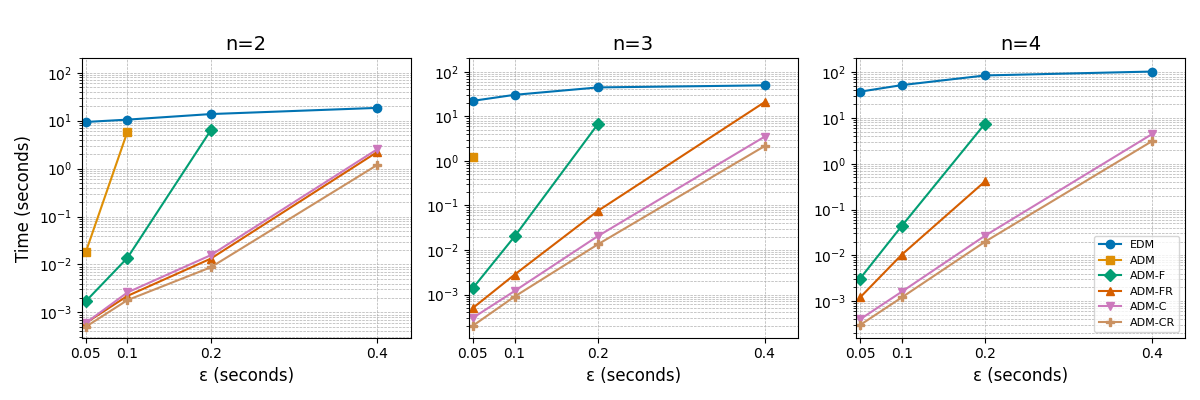
\includegraphics[width=\linewidth]{wt_newnames.png}
		\caption{Running times for monitoring $\varphi_{\text{WT}}$ in log scale. Time limit is 120s, and timed-out instances are not shown.}
		%		\vspace{3mm}
	\end{center}
	%	\vspace{-1em}
\end{figure*}
\begin{figure*}[t]
	\begin{center}
		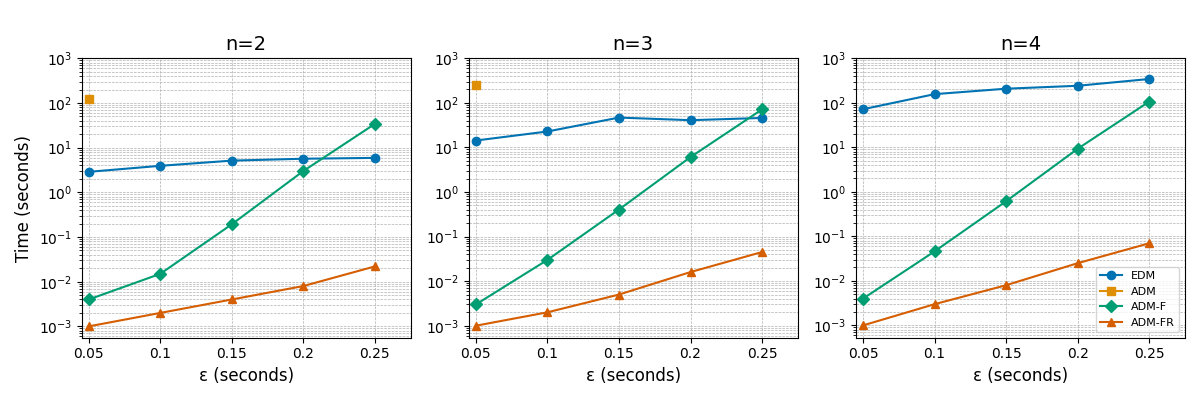
\includegraphics[width=\linewidth]{ms_newnames.png}
		\caption{Running times for monitoring $\varphi_{\text{SD}}$ in log scale. Time limit is 360s, and timed-out instances are not shown.}
	\end{center}
\end{figure*}

%\vspace{-0.5em}
\paragraph*{Water Tank.}
Speedups increase with the number of signals \(n\) and decrease with \(\varepsilon\).
The \textsc{Adm-C} method shows significant improvements over \textsc{Edm}, with up to a $104000\times$ speedup in the best-case (when \(n=4\) and \(\varepsilon=0.05\)) and an $8\times$ speedup in the worst-case (when \(n=2\) and \(\varepsilon=0.4\)).
Note that \(\varepsilon=0.4\) is near the realistic upper limit \cite{MomtazAB23}, indicating no scalability issues.
The \textsc{Adm-Cr} method adds up to a $1.63\times$ speedup over \textsc{Adm-C}.
The \textsc{Adm-Fr} approach significantly improves \textsc{Adm-F}, bringing it below the time-out limit with up to a $476\times$ speedup in non-time-out instances.
As expected, \textsc{Adm} does not perform well.
All methods produce the same verdict for the considered traces.



%\vspace{-0.5em}
\paragraph*{Swarm of Drones.}
Similar to the previous case scenario, speedups in the mutual separation case increase with \(n\) and decrease with \(\varepsilon\).
The \textsc{Adm-Fr} method achieves about a $78000\times$ speedup in the best-case scenario (when \(n=4\) and \(\varepsilon=0.05\)) and a $23\times$ speedup in the worst-case (when \(n=2\) and \(\varepsilon=0.25\)).
The \textsc{Adm-F} method performs slower than SMT in two cases where \(n\) is small and \(\varepsilon\) is large.
%
As in the previous case, \textsc{Adm} does not perform well.
Additionally, \textsc{Adm-C} and \textsc{Adm-Cr} are not applicable here because the arithmetic operations are not monotonic.
Again, all methods yield the same verdicts.

%\vspace{-0.5em}
\paragraph*{Summary.}
%To answer RQ1, we observe that while the speedup achieved with \textsc{Adm} compared to \textsc{Edm} is consistently very high and in three to five orders of magnitude, the tradeoff between efficiency and accuracy depends largely on the type of specifications, the duration of the input signals and the maximal clock skew. The arithmetic and timed operators are particularly sensitive to the over-approximations of \textsc{Adm} and reduce the accuracy of the method. Untimed temporal properties, especially those in which conjunctive and disjunctive operations are not combined, achieve very high levels of accuracy, resulting in an excellent tradeoff. Given the significant increase of efficiency in \textsc{Adm} compared to \textsc{Edm}, the two methods can be effectively combined even in situations where \textsc{Adm} has low accuracy. The combination of \textsc{Adm} and \textsc{Edm} results consistently in the overall increase of efficiency, thus positively answering RQ2.
To answer RQ1, we find that \textsc{Adm} achieves a speedup of three to five orders of magnitude over \textsc{Edm}. However, the efficiency-accuracy tradeoff depends on the type of specifications, input signal duration, and maximal clock skew. Arithmetic and timed operators are particularly affected by \textsc{Adm}'s overapproximations, reducing accuracy. Untimed temporal properties, especially those without mixed conjunctive and disjunctive operations, maintain high accuracy and offer an excellent tradeoff. Despite lower accuracy in some cases, combining \textsc{Adm} and \textsc{Edm} still results in significant gains, positively answering RQ2.
In addition, our incremental monitors scale cleanly to online settings: updates take $O(1)$ time per portion and remain robust to large clock skew, keeping latency within real-time budgets. Consequently, they sustain kHz-level sampling without compromising responsiveness, positively answering the scalability question.

